\chapter{Systemmodelle}

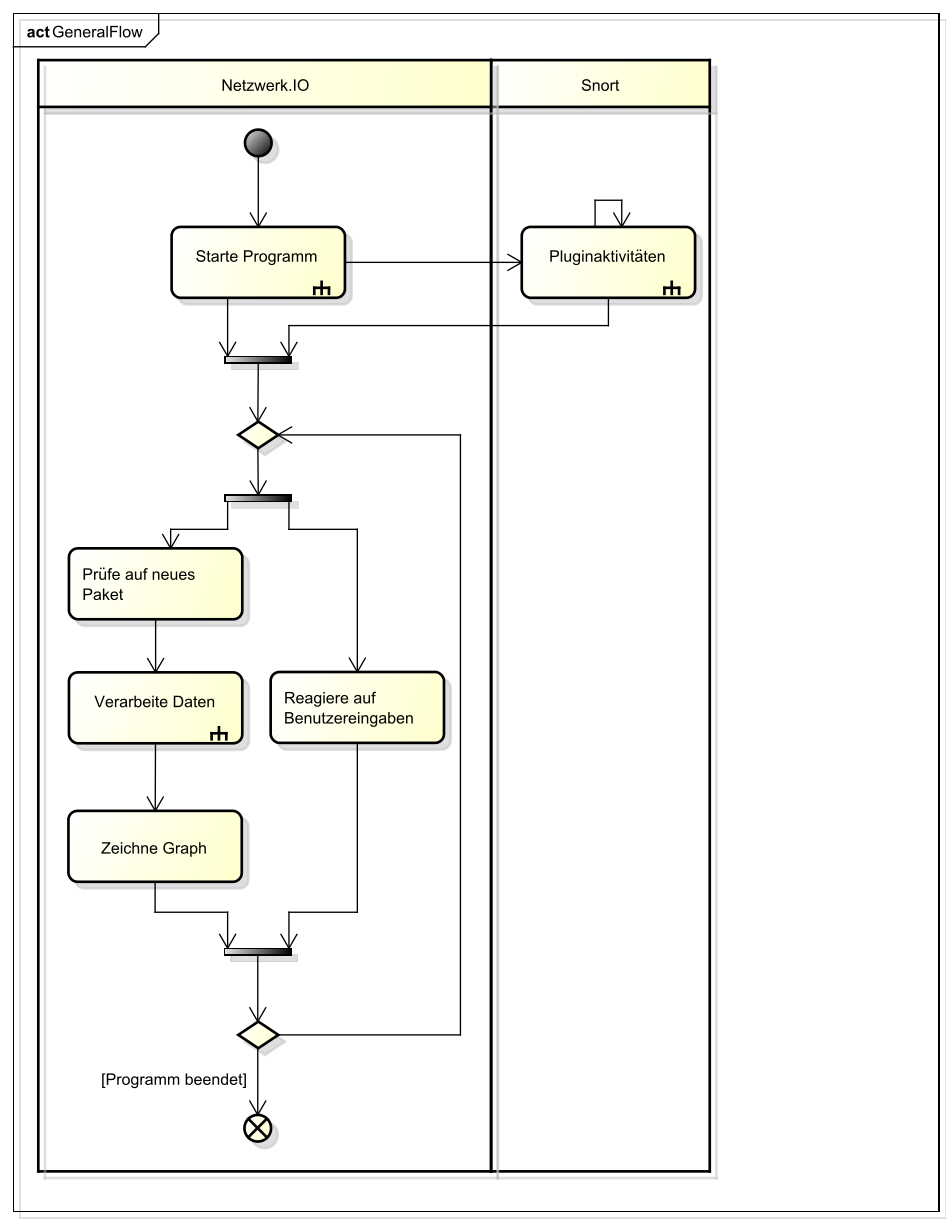
\includegraphics[width=\textwidth]{GeneralFlow}

\section{Szenarien}

\subsection{Szenario 1: Der verhinderte Angriff}

Tom's Firma Insekura nutzt das industrielle Protokoll ProfiNet für die Kommunikation zwischen den Geräten des Systems. Bisher hat Tom keine Möglichkeit gehabt den Netzwerkverkehr zwischen den Drehmaschinen zu kontrollieren. Während des laufenden Betriebs greift der ehemalige Mitarbeiter Udo unbeobachtet auf den Maschinenablauf zu und verursacht dadurch eine Werkzeugkollision. Der materielle Schaden für die Firma ist groß, ein Mitarbeiter wurde leicht verletzt. Zudem kann Tom den Ablauf der Kommunikation und damit die Ursache des Schadens nicht zurückverfolgen.

In der Hoffnung Unfälle und Attacken solcher Art in Zukunft vermeiden zu können, installiert er die freie Software \programname und lässt sie auf einem gut sichtbaren Bildschirm in seinem Büro dauerhaft in Betrieb. Auf dem Display sieht er sämtliche \textbf{Geräte als Knoten} eines Graphen und kann die \textbf{Kommunikationswege zwischen Geräten und Controllern durch gerichtete Kanten} gut verfolgen. In den Einstellungen von \programname \textbf{fügt er den Adressraum des Firmennetzes zu den erlaubten Kommunikationsadressen hinzu}.

Im Laufe der nächsten Tage startet Udo einen weiteren Versuch seiner alten Firma zu schaden. Letztes Mal hat das wunderbar funktioniert, keiner konnte seine fremde Adresse identifizieren und er hatte uneingeschränkte Möglichkeiten falsche Daten an die Drehmaschinen zu übermitteln.

Während sich Udo den Zugang auf das System verschafft, sitzt Tom in seinem Büro und hat seinen Blick gerade auf den Bildschirm mit dem laufenden \programname gerichtet. Er sieht wie ein roter Knoten auf dem Bildschirm erscheint und mit einer der Drehmaschinen beginnt zu kommunizieren. Die Kommunikationskante ist auch rot gekennzeichnet. Sofort eilt Tom zur Tür und drückt auf den Notfall Ausschalter des Systems. Schlimmeres konnte verhindert werden.


\subsection{Szenario 2: Der entlarvte Angreifer}

Im Szenario "Der verhinderte Angriff" wurde beschrieben, wie Tom eine Maschinen Kollision durch die Beobachtung der Kommunikation verhindern konnte. Im Anschluss dieses Vorfalles, erinnert sich Tom, dass \programname eine Funktion zum Auslesen von log Dateien anbietet.

Er öffnet die log Datei des roten Knotens und kann dadurch zurückverfolgen wer den Angriff auf das Firmennetzwerk gestartet hat. Udo steht eine große Schadensersatzklage bevor.
 

\section{Anwendungsfälle} 